\documentclass[11pt, a4paper]{scrartcl} % Packages
%\usepackage{stix}
\usepackage{sansiwona}
\usepackage[margin=1.5in]{geometry}
\usepackage{index}
\makeindex
\usepackage[utf8]{inputenc}
\usepackage[T1]{fontenc}
\usepackage{varwidth}
\usepackage{amsmath, amssymb, amsbsy}
\usepackage{esint}
\usepackage{titlesec}
\usepackage{xcolor}
\usepackage{titling}
\usepackage{braket}
\usepackage{tensor}
\usepackage[linktocpage]{hyperref}
\usepackage{pgfplots}
\usepackage{multicol}
\setlength{\columnsep}{2em}
\usepackage{caption}
\usepackage{amsthm}
\usepackage{import}
\usepackage{cancel}
\usepackage{caption}
\usepackage{tcolorbox}
\usepackage{nicematrix}
\usepackage{mathtools}
\usepackage{enumerate}
\usepackage{graphicx}
\usepackage{lipsum}
\usepackage[italian]{babel}
% To reset footnote numbering each page
\usepackage[perpage]{footmisc}
\usepackage{setspace}
\setstretch{1.2}

%Captions
\captionsetup[figure]{font=footnotesize,labelfont=footnotesize}
\captionsetup[table]{font=footnotesize,labelfont=footnotesize}
%Titlesec
\titleformat{\section}
{\fontsize{15}{20}\sffamily\scshape}
{\normalfont\color{gray}{\fontsize{20}{20}\selectfont\thesection}}
{0.7em}
{}
\hypersetup{colorlinks,breaklinks, linkcolor=[RGB]{74, 122, 164}}

\newcommand\vertarrowbox[3][6ex]{%
  \begin{array}[t]{@{}c@{}} #2 \
  \left\uparrow\vcenter{\hrule height #1}\right.\kern-\nulldelimiterspace\
  \makebox[0pt]{\scriptsize#3}
  \end{array}%
}
\definecolor{asdf}{HTML}{4a7aa4}
% Personalizza la formattazione della subsection
\titleformat{\subsection}[block]{\fontsize{13}{20}\bfseries}{\normalfont\thesubsection}{.5em}{}


% Personalizza la formattazione della subsubsection
\titleformat{\subsubsection}[block]{\fontsize{12}{20}\bfseries}{\normalfont\thesubsubsection}{.5em}{}

% Maketitle customization
\renewcommand{\maketitle}{
\begin{center}
{\sffamily
{\fontsize{20}{20}\selectfont\MakeUppercase\thetitle}}

\vspace{0.2in}

{\large\scshape\sffamily\theauthor}
\end{center}
}

% Titles 
\title{Appunti di Chimica Generale}
\author{Manuel Deodato}
\date{}



%Evaluate symbol
\DeclareMathOperator{\di}{d\!}
\newcommand*\Eval[3]{\left.#1\right\rvert_{#2}^{#3}}

%%%%%%% Numero delle equazioni in formato a.b
\numberwithin{equation}{subsection}
%%%%%

%%%%%%%%%% Personalizzazione numeri lista
\renewcommand{\theenumi}{(\arabic{enumi})}

%%%%%%%%%% Medie con integrali multipli
\def\Yint#1{\mathchoice
    {\YYint\displaystyle\textstyle{#1}}%
    {\YYint\textstyle\scriptstyle{#1}}%
    {\YYint\scriptstyle\scriptscriptstyle{#1}}%
    {\YYint\scriptscriptstyle\scriptscriptstyle{#1}}%
      \!\iint}
\def\YYint#1#2#3{{\setbox0=\hbox{$#1{#2#3}{\iint}$}
    \vcenter{\hbox{$#2#3$}}\kern-.51\wd0}}
\def\longdash{{-}\mkern-3.5mu{-}} 
   % consider using "\mkern-7.5mu" if esint package is loaded
\def\tiltlongdash{\rotatebox[origin=c]{15}{$\longdash$}}
\def\fiint{\Yint\tiltlongdash}

\def\Zint#1{\mathchoice
    {\YYint\displaystyle\textstyle{#1}}%
    {\YYint\textstyle\scriptstyle{#1}}%
    {\YYint\scriptstyle\scriptscriptstyle{#1}}%
    {\YYint\scriptscriptstyle\scriptscriptstyle{#1}}%
      \!\iiint}
      \def\tilongdash{\mkern6mu{-}\mkern-4mu{-}\mkern-5mu{-}} 
   % consider using "\mkern-7.5mu" if esint package is loaded
\def\titiltlongdash{\rotatebox[origin=c]{15}{$\tilongdash$}}
\def\fiiint{\Zint\titiltlongdash}


%%%% Table of contents

\usepackage[titles]{tocloft}

\renewcommand{\cftdot}{}
\usepackage{titletoc}
%\setcounter{tocdepth}{2}

%%%%%%%%%%%%%%%% Toc style

% Personalizzazione scritta indice




% Ambienti
\newtheoremstyle{style1}% name of the style to be used
{15pt}% measure of space to leave above the theorem. E.g.: 3pt
{15pt}% measure of space to leave below the theorem. E.g.: 3pt
{\normalfont}% name of font to use in the body of the theorem
{}% measure of space to indent
{\sffamily\scshape\bfseries}% name of head font
{}% punctuation between head and body
{ }% space after theorem head; " " = normal interword space
{\thmname{#1}\thmnumber{ #2}{\thmnote{~--- #3}}.\newline}

\newtheoremstyle{style2}% name of the style to be used
{15pt}% measure of space to leave above the theorem. E.g.: 3pt
{15pt}% measure of space to leave below the theorem. E.g.: 3pt
{\normalfont}% name of font to use in the body of the theorem
{}% measure of space to indent
{\sffamily\scshape\bfseries}% name of head font
{}% punctuation between head and body
{ }% space after theorem head; " " = normal interword space
{\thmname{#1}\thmnumber{ #2}{\thmnote{~--- #3}}.\ }


\theoremstyle{style2}
\newtheorem{osservazione}{Osservazione}[section]
\newtheorem{esempio}{Esempio}[section]
\newtheorem{esercizio}{Esercizio}[section]
\newtheorem{notazione}{Notazione}[section]

\theoremstyle{style1}
\newtheorem{teorema}{Teorema}[section]
\newtheorem{corollario}{Corollario}[teorema]
\newtheorem{lemma}{Lemma}[teorema]
\newtheorem{definizione}{Definizione}[section]

\renewcommand\qedsymbol{$\blacksquare$}

\newenvironment{svolgimento}{\renewcommand\qedsymbol{$\spadesuit$}\begin{proof}[Svolgimento]}{\end{proof}}

%% Generic box
\newtcolorbox{eqbox}[1][]
{
colback=gray!10,
arc=0pt,
boxrule=0pt,
title=#1
}

 \newenvironment{boxenv}[1][]{
    \begin{eqbox}[#1]
    }{
   \end{eqbox}
}






% Font
\usepackage[osf]{newpxtext}
\usepackage{newpxmath}
%\usepackage{cmupint}
%%%


%%%%%%%%%%%%%%%%%%%%%%%%%%%%%%%%%%%%%%%%%%%%%%%%%%%%%%%%%%%%%%%%%%%%%%%%

\begin{document}
\maketitle
\vspace{9cm}
\begin{figure}[h!]
	\centering
	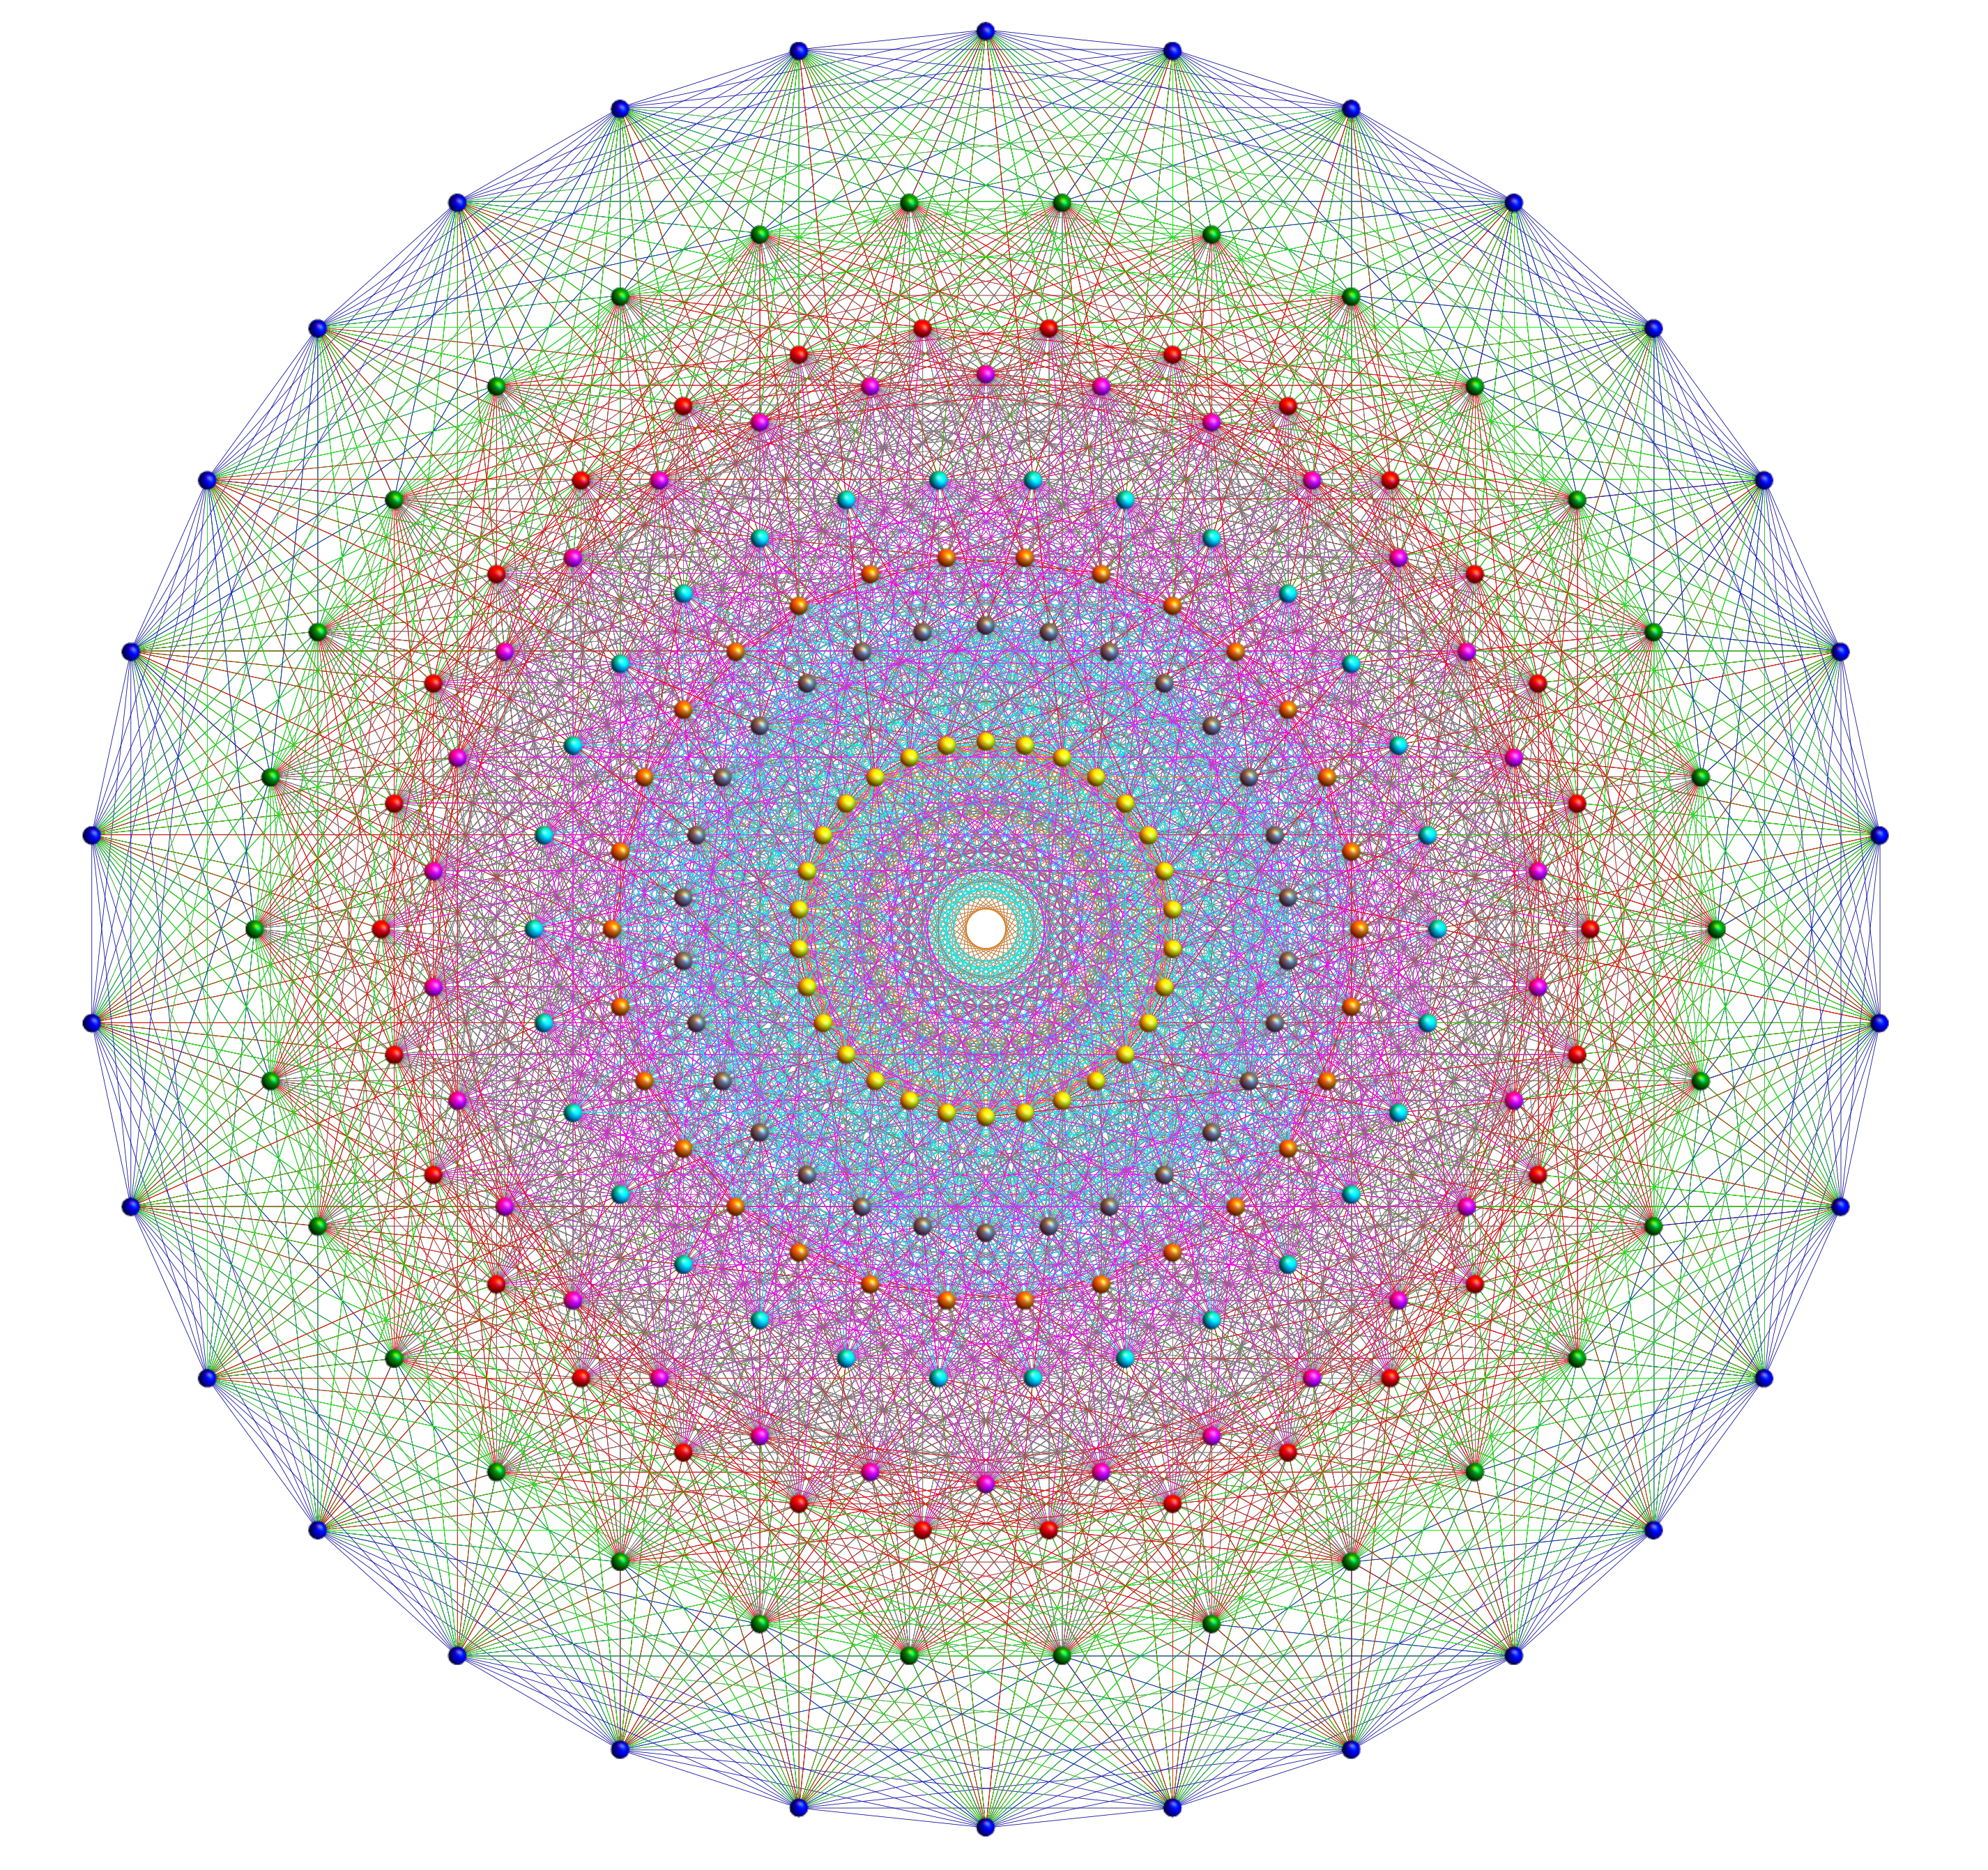
\includegraphics[width=1\columnwidth]{front.jpg}
\end{figure}

\newpage
\tableofcontents 
\newpage
\section{Gli atomi}
\subsection{Osservazione degli atomi}


\subsubsection{Il modello nucleare}
Nel 1987 si ebbe la prima prova dell'esistenza di una struttura interna agli atomi.
Questa deriva dal lavoro con i \textit{raggi catodici} di J. J. Thomson: sottoponendo due elettrodi metallici a elevata differenza di potenziale, si generano raggi catodici; Thomson osserv\`o che questi, immersi in campo elettrico, viravano verso il terminale positivo.
Le particelle che formano questi fasci vennero denominate \textit{elettroni} dopo aver verificato che avevano tutte le stesse propriet\`a indipendentemente dal materiale usato per gli elettrodi dei raggi catodici.

Thomson riusc\`i a misurare il rapporto $e / m_e$, ma la misura separata di carica e massa dovette attendere l'esperimento della goccia d'olio di Milikan. 
Il valore moderno \`e stimato essere $e = 1.602 \cdot  10^{-19} $ C e $m_e = 9.109 \cdot  10^{-31} $ Kg.

Visto che gli atomi risultavano neutri nel complesso, si teorizz\`o conseguentemente la presenza di cariche positive; il modello inizialmente proposto fu il \textit{modello a panettone} di Thomson, successivamente smentito da Rutherford tramite il bombardamento di una lamina di platino con particelle $\alpha $, che si sapevano essere positive e prodotte dal radon.
In questo esperimento, dal modello a panettone, che vedeva gli elettroni immersi in una sorta di gelatina positivamente carica, ci si aspettava una deflessione molto piccola dovuta unicamente alla forza esercitata dagli elettroni.
Quello che si osserv\`o, invece, era che molte particelle $\alpha $ passavano senza essere deflesse, mentre solo alcune lo erano; quello che era estremamente in disaccordo era la deflessione di $180^\circ$ di alcune di queste, cosa non permessa dal modello di Thomson.

A seguito di questo, si teorizz\`o la presenza di un \textit{nucleo} positivamente carico e, lavori successivi, mostrarono che questo nucleo non era composto solo da \textit{protoni}, ma anche da \textit{neutroni}.
\subsubsection{Radiazioni elettromagnetiche}
Per indagare strutture interne di oggetti piccoli come atomi, si usano osservazioni basate sulle propriet\`a della luce emessa da tali oggetti quando soggetti a calore o scarica elettrica.

La luce \`e una forma di \textit{radiazione elettromagnetica}, cio\`e l'insieme di un campo elettrico e un campo amgnetico che oscillano e si propagano nel vuoto alla velocit\`a $c = 3.00 \cdot 10^8 \text{ m}/\text{s}$.
La frequenza di una radiazione si indica con $\nu $ e indica il numero di cicli di radiazione per secondo che passano in un punto dello spazio.
La luce visibile, per esempio, ha $\nu  \sim 10^{15} $ Hz.

Un'onda em ha una sua \textit{ampiezza}, cio\`e la sua altezza rispetto all'asse orizzontale, e il quadrato dell'ampiezza restituisce l'\textit{intensit\`a}.
La lunghezza d'onda $\lambda$, invece, misura la distanza tra due picchi.

Una lunghezza d'onda breve corrisponde ad una frequenza elevata e viceversa; questo \`e esplicitato dalla legge:
\begin{equation}
	\lambda \nu  = c
\end{equation}
\begin{esempio}
La lunghezza d'onda di una radiazione elettromagnetica di frequenza $4.3 \cdot  10^{14} $ Hz \`e data da $\lambda  = \nu  / c = 7.0 \cdot  10^{-7} \text{ m} = 700$ nm.
\end{esempio} 
La lunghezza d'onda della radiazione visibile ha $\lambda \sim 500$ nm: complessivamente, si percepiscono radiazioni nel range $400 \text{ nm} - 700 \text{ nm}$. La luce bianca \`e una miscela di tutte le lunghezze d'onda nel visibile.

La radiazione \textit{ultravioletta} ha $\lambda < 400$ nm, mentre l'\textit{infrarossa} ha $\lambda > 700$ nm.
Le microonde, invece, hanno lunghezze d'onda nel range dei millimetri o centimetri.
\begin{table}[h!]
\centering
\resizebox{\columnwidth}{!}{%
\begin{tabular}{|l|c|c|c|}
\hline
\textbf{Tipo di radiazione} & \textbf{Frequenza ($10^{14}$ Hz)} & \textbf{Lunghezza d'onda (nm)} & \textbf{Energia del fotone ($10^{-19}$ J)} \\
\hline
Raggi $\gamma$             & $>10^6$             & $<0{,}01$              & $>6600$            \\
Raggi X                   & $>10^5$             & $<10$                  & $>660$             \\
Ultravioletto             & $7{,}5 - 30$         & $10 - 400$             & $5 - 124$          \\
Luce violetta             & $7{,}5$             & $400$                  & $5$                \\
Luce blu                  & $6{,}7$             & $450$                  & $4{,}4$            \\
Luce verde                & $5{,}5$             & $550$                  & $3{,}6$            \\
Luce gialla               & $5{,}1$             & $590$                  & $3{,}3$            \\
Luce arancione            & $4{,}8$             & $620$                  & $3{,}1$            \\
Luce rossa                & $4{,}3$             & $700$                  & $2{,}8$            \\
Infrarosso                & $0{,}3 - 4{,}3$      & $700 - 10000$          & $0{,}2 - 2{,}8$    \\
Microonde / Onde radio    & $<0{,}3$             & $>10^6$                & $<0{,}2$           \\
\hline
\end{tabular}
}
\end{table}
\subsubsection{Gli spettri atomici}
Il passaggio di luce bianca attraverso un prisma restituisce uno spettro continuo perch\'e essa \`e composta di tutte le lunghezze d'onda del visibile.
Ripetendo lo stesso, ma con la luce emessa da atomi di idrogeno eccitati, si osserva uno spettro composto da un certo numero di componenti, dette \textit{righe spettrali}; il picco pi\`u luminoso corrisponde alla luce rossa ($\sim 657$ nm).
Questo spettro \`e composto anche da radiazione ultravioletta e infrarossa.

Nel caso particolare dell'idrogeno, le righe spettrali, divise in serie in base alla ragione di spettro a cui appartenevano, si pu\`o riprodurre tramite la formula
\begin{equation}
	\nu  = \mathcal{R} \left\{ \frac{1}{n_1^2}- \frac{1}{n_2^2} \right\} , \ n_1 = 1,2,\ldots, \ n_2 = n_1+1, n_1+2, \ldots
\end{equation}
con $\mathcal{R} = 3.29 \cdot  10^{15} $ Hz \textit{costante di Rydberg}.
In particolare, la \textit{serie di Balmer} si trova nel visibile e poco sopra ed \`e relativa a $n_1=2$; la \textit{serie di Lyman} si trova nell'ultravioletto ed \`e relativa a $n_1=1$.

\begin{esempio}
Prendendo $n_1=2$ e $n_2=3$, sa di trovarsi nella serie di Balmer; pi\`u esattamente
\[
\nu  = \frac{5}{36}\mathcal{R} \implies \lambda = \frac{c}{\nu }= \frac{36}{5} \frac{c}{\mathcal{R} } \approx 657 \text{ nm}
\] 
quindi corrisponde alla riga rossa nello spettro dell'idrogeno.
\end{esempio}
Lo \textit{spettro di assorbimento} di un elemento \`e ottenuto osservando la luce rimanente dopo che la luce bianca ha attraversato un vapore di tale elemento.
Questo \`e composto da una serie di righe nere relative alle frequenze che quel tale elemento \`e ing rado di emettere.

\subsection{La teoria quantistica}


\end{document}
